\section{U001 Hybrid matrix and vector coordination}
\label{sec:u001}

A matrix engine can finish useful work only as quickly as the surrounding computation supplies its inputs and consumes its outputs. Attention makes this dependence particularly visible: a matrix multiplication produces scores, vector and reduction operations turn the scores into probabilities, and another matrix multiplication consumes them. An accelerator therefore needs more than a fast matrix datapath. It needs an execution contract that connects different operation shapes, readiness conditions, storage owners, and completion events without imposing avoidable waiting. The question in U001 is which granularity exposes useful overlap, who manages that overlap, and what the resulting control costs are.

This is a mechanism comparison. The NVIDIA case is principally Hopper and a pinned FlashAttention-3 kernel; a separate paragraph identifies a relevant Blackwell change. Ascend A2 and the newer 3510 architecture are kept distinct. The TPU case uses the public Pallas programming model rather than an invented description of a proprietary instruction scheduler. Tenstorrent is considered through its documented compute and circular-buffer interfaces. Our superscalar NPU, abbreviated SSNPU, is discussed through the supplied source-inspection record of a particular timing model, not as measured silicon. Published Groq designs provide a further comparison point. None of the mechanisms described here establishes a performance ordering between platforms.

\subsection{The algorithm creates several different dependencies}

For one query block, let $Q\in\mathbb{R}^{B_q\times d}$ and let the $j$th key and value blocks be $K_j\in\mathbb{R}^{B_k\times d}$ and $V_j\in\mathbb{R}^{B_k\times d_v}$. The score block is
\begin{equation}
 S_j=\alpha QK_j^{\mathsf T}+M_j,
\end{equation}
where $M_j$ expresses the selected mask. A convenient online formulation retains a row maximum $m_j$, a row denominator $\ell_j$, and an unnormalized output accumulator $O_j$. With rowwise broadcasting understood, one iteration is
\begin{align}
 m_j &= \max\bigl(m_{j-1},\operatorname{rowmax}(S_j)\bigr),\\
 a_j &= \exp(m_{j-1}-m_j),\qquad
 P_j=\exp(S_j-m_j),\\
 \ell_j &= a_j\ell_{j-1}+\operatorname{rowsum}(P_j),\\
 O_j &= a_jO_{j-1}+P_jV_j.
 \label{eq:u001-online-attention}
\end{align}
For rows with valid scores, the recurrence starts from $m_0=-\infty$, $\ell_0=0$, and $O_0=0$, with the first valid block handled consistently with those initial values. The final output divides each row of $O_j$ by its corresponding denominator. This mathematical formulation does not prescribe a particular instruction schedule or numerical implementation. Input precision, accumulator precision, approximation of exponential, exceptional values, and the treatment of fully masked rows must be specified separately.

There are at least three kinds of dependence in this small program. Within a block, probabilities require the appropriate maximum, and the contribution to the output requires those probabilities. Across blocks, the running state connects successive iterations. Across query rows or independent heads, substantial work can be independent. These distinctions explain why both of the following statements can be true: a score block cannot skip its softmax dependencies, and a kernel can execute some matrix work concurrently with softmax work. FlashAttention-3 explicitly exploits asynchronous matrix execution and rearranged block scheduling to obtain such overlap on Hopper. Its reported performance is evidence for its evaluated configurations, not a transferable result for the SSNPU or for every attention shape.~\citep{u001-fa3}

The decomposition also prevents a misleading account of ``the vector stage.'' Row maximum, exponential, sum, broadcast, output rescaling, and normalization have different input requirements. A row maximum can accumulate partial maxima as score fragments arrive, but its final value requires every active fragment in that reduction domain. An elementwise operation with independent inputs may become eligible much earlier. The relevant dependency is therefore a relation between producer regions and consumer operations, not merely an arrow between two large boxes labelled matrix and vector.

\subsection{Five granularities must be distinguished}

We use five separate meanings of granularity. \emph{Semantic work granularity} is the operation the program expresses, such as a score tile or row reduction. \emph{Dispatch granularity} is the unit admitted or selected by a scheduler. \emph{Readiness granularity} is the smallest region for which the implementation can establish that required data are valid. \emph{Synchronization granularity} is the participating group and event scope used to communicate this fact. \emph{Transfer granularity} describes a memory request or movement unit. These quantities can differ within one operation and can change between generations of the same product.

For example, the supplied benchmark inspection identifies a group score tile with $B_q=B_k=128$, but the selected four-PE kernel gives each PE a $32\times128$ FP32 score shard. The group FP32 payload is $64$ KiB, the per-PE payload is $16$ KiB, and a modeled vector readiness cell is $128$ bytes. A cell contains $32$ FP32 values by capacity; it is neither the whole vector operation nor evidence that those values execute in one cycle. Doubling $B_k$ doubles the shard's logical byte count without proving that dispatch or readiness granularity changes. These are source-derived geometry observations and arithmetic, not dynamic instruction counts.~\citep{u002-benchmark-fa,u001-ssnpu-audit}

A corresponding NVIDIA example must name its own layer. A full warp executing one FP32 operation per active thread spans $128$ bytes per operand when all $32$ threads participate. Hopper WGMMA instead uses a warpgroup of $128$ cooperating threads. For a dense BF16 $m64n128k16$ operation, the logical inputs contain $2$ KiB of A and $4$ KiB of B, while an FP32 accumulator contains $32$ KiB. These figures describe matrix shapes and representations, not memory transactions or a universal software tile.~\citep{u001-ptx} Equal byte counts between an SSNPU cell and a warp operand establish no equivalence between their scheduling semantics.

The historical Ascend attention design also identifies an operator whose vector piece is $8\times1024$ FP32, or $32$ KiB. Its significance is a buffer and decomposition choice in that operator, not a fixed hardware asynchronous scheduling quantum.~\citep{u001-ascend-fa-design} Comparing this piece directly with a GPU warp or a $128$-byte readiness cell mixes semantic work, capacity, and execution participation. A meaningful comparison first identifies the producer region, the required consumer region, and the actual operation that moves or consumes it.

\subsection{What finer readiness can and cannot change}

Consider an illustrative producer that makes four independently usable regions available at times $t_1<t_2<t_3<t_4$. A consumer requires only the first region. If the interface exposes one whole-tile completion event, the earliest dependency-permitted start is $t_4$. If it exposes correct region readiness, that bound becomes $t_1$. The opportunity is $t_4-t_1$, but the actual improvement can be smaller or zero: the execution unit may be occupied, a destination may be unavailable, or bank conflicts may prevent admission. This is a dependency argument, not a prediction of observed cycles.

For a consumer $v$, write its earliest admissible start schematically as
\begin{equation}
 s_v\geq\max\{r_v,\ d_v,\ e_v,\ b_v,\ o_v\},
 \label{eq:u001-admission}
\end{equation}
where $r_v$ is the latest required input-ready time, $d_v$ is destination availability, $e_v$ is execution-resource availability, $b_v$ is the relevant bank or port availability, and $o_v$ expresses ordering constraints. Replacing whole-tile readiness with region readiness changes $r_v$ only. A scheduling proposal that ignores the other terms can substantially overstate its benefit.

\begin{figure}[tb]
\centering
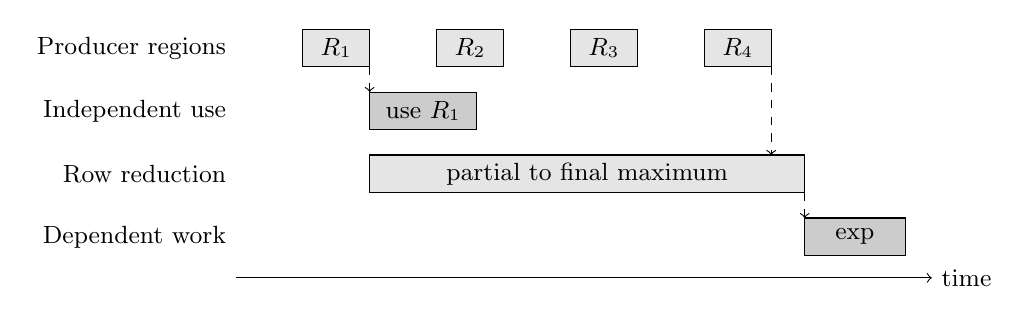
\begin{tikzpicture}[x=0.85cm,y=0.8cm, every node/.style={font=\small}]
 \node[anchor=east] at (0,3) {Producer regions};
 \node[anchor=east] at (0,2) {Independent use};
 \node[anchor=east] at (0,1) {Row reduction};
 \node[anchor=east] at (0,0) {Dependent work};
 \draw[->] (0,-0.65)--(10.4,-0.65) node[right] {time};
 \foreach \x/\n in {1/1,3/2,5/3,7/4} {
   \draw[fill=black!10] (\x,2.7) rectangle (\x+1,3.3);
   \node at (\x+0.5,3) {$R_{\n}$};
 }
 \draw[fill=black!20] (2,1.7) rectangle (3.6,2.3);
 \node at (2.8,2) {use $R_1$};
 \draw[->,dashed] (2,2.7)--(2,2.3);
 \draw[fill=black!10] (2,0.7) rectangle (8.5,1.3);
 \node at (5.25,1) {partial to final maximum};
 \draw[->,dashed] (8,2.7)--(8,1.3);
 \draw[fill=black!20] (8.5,-0.3) rectangle (10,0.3);
 \node at (9.25,0) {exp};
 \draw[->,dashed] (8.5,0.7)--(8.5,0.3);
\end{tikzpicture}

\caption{Conceptual readiness relationships. Region arrival can advance independent work and partial reduction, while the final maximum still gates dependent exponentials in this formulation. Horizontal distances are illustrative and do not represent measured timing or a particular architecture.}
\label{fig:u001-readiness}
\end{figure}

Now make each region one quarter of a softmax row. Partial maxima can begin early, but exponentiating every quarter relative to the final block maximum cannot begin merely because the first quarter exists. One may use an alternative online update scheme, but then its additional rescaling and retained state belong in the accounting. Alternatively, make each region a complete subset of rows. Those rows can complete their reductions without waiting for unrelated rows, provided the producer really finishes the corresponding reduction dimension and the consumer mapping supports that partition. Fine readiness is valuable when it matches the algorithm's independence; an arbitrary byte partition does not create such independence.

This distinction also matters for low-concurrency workloads. Let $N$ be the number of useful pipeline iterations, $T_{\mathrm{fill}}$ the initial preparation interval, $I$ the achievable steady-state initiation interval, and $T_{\mathrm{drain}}$ the remaining work after the final iteration is admitted. An idealized latency decomposition is
\begin{equation}
 T(N)=T_{\mathrm{fill}}+(N-1)I+T_{\mathrm{drain}},\qquad N\geq1.
\end{equation}
Reducing $I$ has little leverage when $N=1$. Reducing a real dependency on the first or last tile can instead affect fill or drain. Conversely, splitting work more finely can increase setup, events, and intermediate storage. A claim about short-task latency must state batch size, heads, sequence lengths, dimensions, masking, and partitioning; it cannot be inferred from a steady-state utilization number or generalized to all decode.

\subsection{NVIDIA assigns roles in software and eligibility in hardware}

Hopper exposes asynchronous matrix and transfer facilities that a compiler or kernel author can compose into a fused pipeline. TMA moves appropriately described tensor data, while warps and warpgroups perform different producer and consumer roles. Hardware schedules eligible resident work and enforces exposed completion mechanisms; software determines tile shapes, layouts, stage count, role assignment, and synchronization placement. The Hopper tuning guide describes the hardware facilities, while a concrete kernel establishes how they are used.~\citep{u001-hopper}

CUTLASS's Hopper organization makes this division explicit. Producer warps wait for an empty shared-memory stage, initiate a transfer, and associate arrival with the stage's completion state. Consumer warps wait for the stage to become full, issue matrix work, and release the stage when it can safely be overwritten.~\citep{u002-cutlass} This is already dynamic readiness-based coordination at the software-defined stage boundary. It should not be described as a machine that relies entirely on a fixed cycle schedule, nor should ready-warp scheduling be equated with unrestricted CPU-style speculative out-of-order execution.

The useful opportunity is to overlap independent stages and to use different engines concurrently. The cost includes producer instructions, barrier state, register and shared-memory capacity, layout preparation, and constraints on resident work. More software stages can improve latency tolerance while reducing other forms of concurrency. An application-level runtime can also select different decompositions: TensorRT-LLM documents multi-block attention choices intended to provide additional work when batch-times-head count is small. That option introduces its own partial-result and coordination costs; it is a relevant baseline for a low-concurrency comparison, not a guarantee of lower latency.~\citep{u001-trt-attention}

The generation boundary is important. Blackwell SM100 introduces the \texttt{tcgen05} family with single-thread matrix instruction launch and Tensor Memory for accumulators.~\citep{u001-tcgen05} FlashAttention-4 describes algorithm and pipeline changes for that organization.~\citep{u001-fa4} Therefore the number of threads participating in Hopper WGMMA cannot be presented as an immutable property of NVIDIA matrix execution. A fair comparison may choose Hopper for its pinned implementation evidence, but it must say so rather than treating an older interface as the only available GPU approach.

\subsection{Ascend exposes pipeline and inter-core coordination}

In the A2 separated organization, Cube and Vector cores have independent scalar control. The documented architecture distinguishes Cube operand and accumulator storage from the Unified Buffer used by Vector work; movement engines connect the relevant storage levels. Its instruction queues and synchronization interfaces permit overlap across pipelines while preserving dependencies. GM-addressed exchange is not synonymous with a mandatory HBM round trip because the architecture documents L2 caching of DMA traffic.~\citep{u001-ascend-basic}

At the algorithm and compiler level, host tiling and kernel code choose which Cube region becomes which Vector pieces, which layouts are used, and how much state remains resident. At the API level, queues and events identify ownership and inter-pipeline dependencies. Hardware executes those operations and supplies the movement and event mechanisms. A larger Cube tile can amortize setup and reuse operands, while smaller Vector pieces can begin useful work incrementally. Neither choice is free: exchanged data, local capacity, events, and the number of simultaneously live intermediates constrain the resulting schedule.

The \texttt{TQue} contract is especially relevant because it separates a queue of tensor references from the number of physical buffers allocated for that queue. Queue depth and multibuffering count answer different questions; increasing one does not automatically increase the other.~\citep{u002-ascend-tque} This is a concrete example of why an API-level queue size cannot serve as a universal hardware issue granularity. Similarly, an operator's $32$ KiB vector allocation is not evidence that every useful handoff waits for $32$ KiB.

For architecture 3510, the official specification identifies additional L0C-to-UB and UB-to-L1/L1-to-UB paths, as well as SSBuffer for AIC--AIV communication. It also documents SIMD register-based execution and SIMT hardware, including warp schedulers, so an A2 description must not be treated as the execution model of every Ascend generation.~\citep{u001-ascend-3510} These changes alter the possible handoff and control costs. The present comparison does not project A2's paths onto 3510, infer throughput from the existence of a path, or assume that every software release uses it optimally. The open measurement question is which decomposition sustains useful overlap for the selected shapes after exchange and control costs are included.

\subsection{TPU gives the compiler a larger scheduling responsibility}

Pallas describes a TPU TensorCore with scalar, vector, and matrix execution resources that can operate asynchronously under compiler management. The programmer sees a predominantly single-threaded program and can express DMA, memory spaces, and pipeline structure.~\citep{u001-pallas-pipeline} This organization separates an instruction stream's presentation from the concurrency of the engines it controls. A sequential kernel body does not imply that every transfer, matrix operation, and vector operation is serialized to completion.

The compiler and kernel author choose blocking, layout, fusion, and the order of work; explicit buffer and semaphore operations establish important readiness conditions. The documented constraints on blocks and memory spaces, and the distinction between vector and matrix operations, matter when mapping a score tile to reductions.~\citep{u001-pallas-details} A pipeline that overlaps HBM-to-VMEM DMA with computation does not by itself establish that the score matrix multiply overlaps every softmax stage. That requires an effective schedule and sufficiently independent work on the relevant engines.

A static description of that schedule should not be caricatured as an inability to handle runtime variation. Pallas supports scalar-prefetched information for runtime block indexing in documented sparse patterns.~\citep{u001-pallas-sparse} Runtime completion and buffering can handle lateness by waiting rather than by corrupting data. The likely tradeoff, as a design inference, is between predictable scheduling with relatively explicit lifetimes and the ability to exploit unanticipated ready work. Which side matters more depends on shape regularity, memory behavior, the compilation, and available local capacity. It is not determined by the label ``compiler directed.''

\subsection{Tenstorrent separates placement from readiness}

Tenstorrent's Metalium programming model divides work among data-movement and compute roles. RISC-V control processors issue commands; the tensor arithmetic is performed by the corresponding compute engines. Circular-buffer operations coordinate publication, consumption, and available space.~\citep{u001-metalium} Software placement of kernels and streams therefore coexists with runtime readiness and backpressure. A static placement is not necessarily a cycle-by-cycle static execution schedule.

Within Tensix, the matrix engine and vector engine meet through Dst storage. Unpack, math, and pack activities have explicit ownership synchronization; the documented \texttt{tile\_regs\_*} lifecycle separates acquiring compute access, committing results, waiting for packing access, and releasing the resource.~\citep{u001-tensix} The implication for attention is that local ownership can be as important as nominal engine independence. Two operations assigned to different arithmetic facilities may still serialize because their command role, Dst region, or packing path is shared.

The official repository's investigation of SDPA implementation paths distinguishes a non-streaming FP32-Dst path, where the math-thread exponential serializes with matrix work, from a streaming path that issues exponential work from the pack thread.~\citep{u001-tt-sdpa-investigation} This is useful implementation-specific evidence, not proof that all Tensix kernels either overlap or fail to overlap matrix and vector work. The algorithm must still provide independent blocks; the kernel must provide compatible Dst ownership and command sequencing; and L1 circular buffers must support the required run-ahead. Host asynchronous dispatch or replay cannot establish any of those internal overlap properties by itself.

The published Groq TSP designs show a further possible division of responsibility: compiler placement and timing arrange streams between functionally specialized slices, with network synchronization maintaining the timing contract.~\citep{u001-groq2020,u001-groq2022} This can make predictable streaming attractive, but it does not remove the attention dependencies derived above. These published designs are a comparison of contracts, not a description of every current Groq product or a low-concurrency performance verdict.

\subsection{The SSNPU opportunity is bounded dynamic coordination}

The supplied SSNPU audit covers the handwritten TimingSim snapshot at commit \texttt{d5419b3e721d}. It observes logical operand tags, whole-tile readiness, conditional cell readiness, bounded issue queues, resource checks, and physical binding. CUBE selection is gated by dependence, chain order, speculation, and execution or storage resources. VEC selection is organized by execution class and is subject to initiation intervals, destination capacity, and backpressure. Cell-mode vector block entry retains an ordering restriction.~\citep{u001-ssnpu-audit} These facts support a bounded dynamic coordination design; they do not describe unrestricted global out-of-order execution.

The intended division is that software expresses operation geometry, layouts, logical dependencies, and reuse, while the hardware model enforces eligible readiness and resource admission. Conditional cell readiness can lower $r_v$ in Equation~\ref{eq:u001-admission} for supported producer--consumer combinations. It cannot lower the other admission bounds automatically, and an operation requiring whole-tile readiness remains constrained by that contract. The audit does not establish arbitrary nonlinear layouts, arbitrary independent source shapes, or an automatically optimal compiler decomposition.

The corresponding normative design requirement is precise: every early consumer must read the correct generation of every required region, no consumer may observe an unfinished or overwritten value, and issue must respect both program ordering and physical resource ownership. This requirement is independent of the particular mechanism used to implement it. Logical tags, scoreboards, readiness masks, bank reservations, and queue selection are implementation choices that carry state, wiring, arbitration, and verification obligations. An abbreviated source program cannot demonstrate that their total cost is lower than that of explicit software stages.

The target architecture should also be kept distinct from a narrow executable snapshot. Functionality delivered by a submitted change belongs in the after-merge target when the change is integrated; its absence from an earlier experiment does not establish architectural inexpressibility. Conversely, a proposed interface does not prove that the measured path used it. For U001, this distinction requires the exact build and configuration before attributing any overlap to cell readiness, ready bypass, or a particular binding path. TimingSim observations are not evidence of complete RTL integration, clock closure, physical area, or energy.

\subsection{A useful evaluation isolates the source of overlap}

A matched study should retain the same attention semantics and vary query rows, key length, head dimensions, masking, and available independent heads. It should record semantic tiles, per-owner shards, readiness regions, synchronization participants, and transfer units separately. End-to-end latency should include preparation, fill, steady state, and drain. A steady-state engine-utilization trace should identify what useful work overlaps, rather than merely showing two queues nonempty.

For the SSNPU, a readiness-granularity ablation must preserve the rest of the build, resource budget, scheduling options, and numerical path. Otherwise a change attributed to smaller regions may instead come from different reduction ordering, queue policy, or storage capacity. Competent GPU, Ascend, TPU, and Tenstorrent baselines should use their own supported fusion and pipelining facilities. The resulting ledger must include event and issue work, retained payload, extra transfers, mapping and arbitration state, and correctness and progress constraints. Finer granularity is justified when it advances useful admissible work enough to repay those costs; neither finer readiness nor a larger matrix tile is intrinsically better.
